\documentclass[11pt]{article}
\usepackage{geometry}                % See geometry.pdf to learn the layout options. There are lots.
\usepackage[parfill]{parskip}
\usepackage{graphicx}
\usepackage{amsmath, amsthm, amssymb}
\usepackage{epstopdf}
\DeclareGraphicsRule{.tif}{png}{.png}{`convert #1 `dirname #1`/`basename #1 .tif`.png}
\usepackage[utf8]{inputenc}
\usepackage[english]{babel}

\newtheorem{theorem}{Theorem}
\newcommand{\be}{\begin{equation*}}
\newcommand{\ee}{\end{equation*}}
\newcommand{\bee}{\begin{eqnarray*}}
\newcommand{\eee}{\end{eqnarray*}}

\title{Dodonaphy Notes}

\begin{document}
\maketitle
\section{Abstract}
Hyperbolic spaces allow quality embeddings of nested data structures, such as trees.
Recent efforts to embed phylogenetic trees using distance-based optimisation demonstrate promising results for embedding single trees.
However, expressing uncertainty in phylogenetics involves a probability distribution over a super-exponential number of trees.
Here, using low dimensional hyperbolic tree embeddings, we explore the Bayesian posterior distribution of trees in a continuous manner.
First, we empirically demonstrate that a posterior surface can be well approximated with tree embeddings using an MCMC in the embedding space.
We also evaluate the potential of variational inference in the embedding space.

\section{Hyperbolic Space}
The Poincaré ball $\mathbb{P}^{d} = \{x\in \mathbb{R}^{d} \,:\, ||x||<1\}$ models hyperbolic space $\mathbb{H}^{d}$ using the metric:
\begin{equation*}\label{eq:poin_dist}
d(x,y) = \textnormal{arccosh}\Big(1 + 2 \frac{||x-y||_{2}^{2}}{ (1-||x||_{2}^{2}) (1-||y||_{2}^{2})}\Big),
\end{equation*}
where $||x||_{2}$ is the $l^{2}$-norm in $\mathbb{R}^{d}$.

\section{Hyperbolic Embeddings}
We form continuous embeddings of trees using one point in the Poincare ball $\bold{x} \in \mathbb{P}^{d}$ for each node in the tree.
For an unrooted tree with $S$ taxa, there will be $m=2S - 2$ nodes locations $\bold{X} \in(\mathbb{P}^{d})^{m}$, where $\bold{X} = \{\bold{x}_{i}: i=1, ..., m\}$.
Embedded nodes are connected to form the minimum spanning tree (MST) protocol that ensures internal nodes have three neighbours and tip nodes have one neighbour.
Both the branch lengths and tree topology may freely change as nodes move.
Once a tree $T(\bold{X})$ is formed, its prior probability $p(T)$ and the likelihood of a sequence aligmnent p(D\big|T) under a given model and data $D$ may be easily determined.

This method is quite distinct from cost functions that are based on pair-wise distances. For example Chami's variant on Dasgupta's cost, the log-a-like used by Wilson or see refs in Chami. Here, nodes placements do not directly contribute to the cost function (tree posterior), they only impact how a tree is formed. The point of using $\mathbb{H}^{n}$ is to exploit its geometry as a way to move between ``adjacent'' trees.

Not every tree may be accessible under this MST protocol and in this sense, we have a variational distribution over trees.
For example, under a MST it would not be possible to join two very distant edges joined directly if there is an available intermediary node.
This raises an interesting question: given a connection protocol, is there a limit to the trees that can be generated?

\section{MCMC}
Since each set of node embeddings corresponds to a tree which has a well defined likelihood and prior probability, MCMC can proceed with the standard Metropolis-Hastings algorithm.
The set of nodes are initialised to locations $\bold{X}_{0}$.
For each node $\bold{x}_{i} \in \bold{X}_{0}$ a new location is proposed and accepted or rejected according to the Metropolis-Hastings algorithm, giving the next iteration $\bold{X}_{1}$.

We propose a node's new location from a Gaussian by projecting the point from the Poincare ball into $\Psi: \mathbb{P}^{d} \to \mathbb{R}^{d}$.
First project onto the hyperboloid model in $\mathbb{R}^{d+1}$ using $\phi(\bold{x}_{i})$ (see appendix), then projecting onto the tangent plane of $\bold{x}=0$ using the $d$-dimensional vector $u=(0, 1, 1, 1,...)$: $\Psi(\bold{x}_{i}) = \psi(\bold{x}_{i}) \cdot u $.
A new point is drawn from a Gaussian located at $\Psi(\bold{x}_{i})$ with given standard deviation, before being projected back to the Poincare ball with $\Phi^{-1}$.

\subsection{Continuity}
Under a MST protocol, the total length of the tree is continuous as nodes move.
As a node $\bold{x}_{i}$ moves continuously:
\begin{itemize}
\item Case (1) the tree does not change topology. The branch lengths of node $i$ change continuously and so the total length $\ell$:
\be
\dfrac{\partial \ell}{\partial \bold{x_{i}}} = cst.
\ee
\item Case (2) the tree changes topology. Suppose $x_{i}$ moves through the point $a$ and the topology changes from $\tau_{1}$ to $\tau_{2}$. The limit from the first topology $\text{lim}_{x_{i} \to a^{\tau_{1}}} \ell = \text{lim}_{x_{i} \to a^{\tau_{2}}} \ell$.
\end{itemize}

If the distance between every pair of two nodes $d(i,j)$ accurately reflects the number of mutations per site $\nu_{ij}$ between the two, then under a JC69 model, the total branch length $\ell$ uniquely determines the likelihood function $p(D|T)$.
\[
P(\nu_{ij}) = 
\begin{cases}
	\frac{1}{4} + \frac{3}{4} e^{\nu_{ij}} & i \neq j\\
	\frac{1}{4} - \frac{1}{4} e^{\nu_{ij}} & i = j
\end{cases}
\]
% TODO: show
%The likelihood 
%\bee
%p(D, T) &=& [\sum_{x\in\{A,C,T,G\}} P_{sx}(d_{o_{1}}) L^{o_{1}}(x)][...]\\
%&=& [4 P_{sA}(d_{o_{1}}) L^{o_{1}}(A)][...]
%\eee
The difficulty is to get the pairwise distances to match the number of mutations per site.
% prior?

\section{Variational Inference}
In VI, the posterior surface (here a set of surfaces --- one for each embedded node $i$) is approximated by a variational distribution $q_{i}(z_{i})$, each parameterised by parameters $z_{i}$.
When the data $D$ is fixed, minimising the KL divergence to the posterior $\text{KL}({\bf q}(\phi)||p(T\big|D))$ is equivalent to maximising the evidence lower bound (ELBO):
\be
\text{ELBO}(q) = \mathbb{E}_{q}[\log(p(z,D))] - \mathbb{E}_{q}[\log(q(z))].
\ee
Working with the ELBO is computationally advantageous since it does not depend on the intractable marginal distribution of the data $p(D)$, which is involves integrate over all tree topologies and all branch lengths.
We consider two mean-field variational distributions for the node locations in $\mathbb{P}^{d}$: a logit-Normal distribution and a ``wrapped'' Normal distribution as proposed in \cite{Nagano2019Wrapped}.

In both these approaches, the variational distribution $\bold{q}$ is smooth, however the posterior probability is not guaranteed to be continuous let alone differentiable as the topology changes.
However this difficulty is partly overcome since the ELBO is not a point estimate, but is an expectation taken from $k$ samples.
Any discontinuities in $p(z,D)$ are smoothed through sampling under $q$.

To optimise the elbo we use stochastic gradient ascent implemented in PyTorch.
The autograd functionality of PyTorch automatically computes the gradient of the elbo in order to stochastically optimise with gradients.

Since the ELBO is an expectation under $q$, which in this case is a vector of normal distributions $g(x)$,
\bee
\text{ELBO}(q) &=& \mathbb{E}_{q}[\log(p(z,D))] - \mathbb{E}_{q}[\log(q(z))]\\
&=& \int_{\mathbb{R}^{d}}[\log(p(z,D))] d\bold{q} - \int_{\mathbb{R}^{d}}[\log(q(z))] d\bold{q}\\
&=& \int_{\mathbb{R}^{d}}[\log(p(z,D))] \circ g(z) dz - \int_{\mathbb{R}^{d}}[\log(q(z))] \circ g(z) dz.
\eee
% TODO: make clear
Since g(z) is infinitely differentiable and
\be
\dfrac{d}{dz_{i}} (f \circ g) = f \circ \dfrac{dg}{dz_{i}},
\ee
we find that the elbo is also infinitely differentiable.



\section{Results}
As a toy example, a posterior was approximated for a six taxa set using Dodonaphy's MCMC and its VI before being compared to BEAST2 --- an established MCMC software.
A tree was simulated using a birth (rate $2$) death (rate $.5$) model and a sequence alignment was generated from this tree under the JC69 model of genetic evolution.
The pairwise patristic distances were computed between the tips on the simulated tree.
The tips were initialised in the Poincare ball using hydra.
Then the internal nodes were randomly placed in $\mathbb{P}^{d}$ with uniform directional and radius from a scaled Beta distribution $ r \sim s \times \text{Beta}(a=2, \beta=5)$ using scales $s \in [0, 2*\min(d(0, \bold{x}_{i})]$, where $i$ only includes the tip nodes.
Internal node locations were sampled $10^{4}$ times and the initialisation with the highest tree likelihood was selected.

\subsection{MCMC}
The final log likelihood from BEAST was -6280 (similar to it's log posterior of -6271). In comparison, Dodonaphy MCMC gave -6280, which is a close match.
However, figure~\ref{fig:stat_cmp}a illustrates that samples from Dodonaphy's MCMC always gave one incorrect split.
This could indicate that the MCMC chain is stuck in a local optima and that techniques like using Metropolis-coupled MCMC to escape this optima should be employed.

\begin{figure}[htbp]
\begin{center}
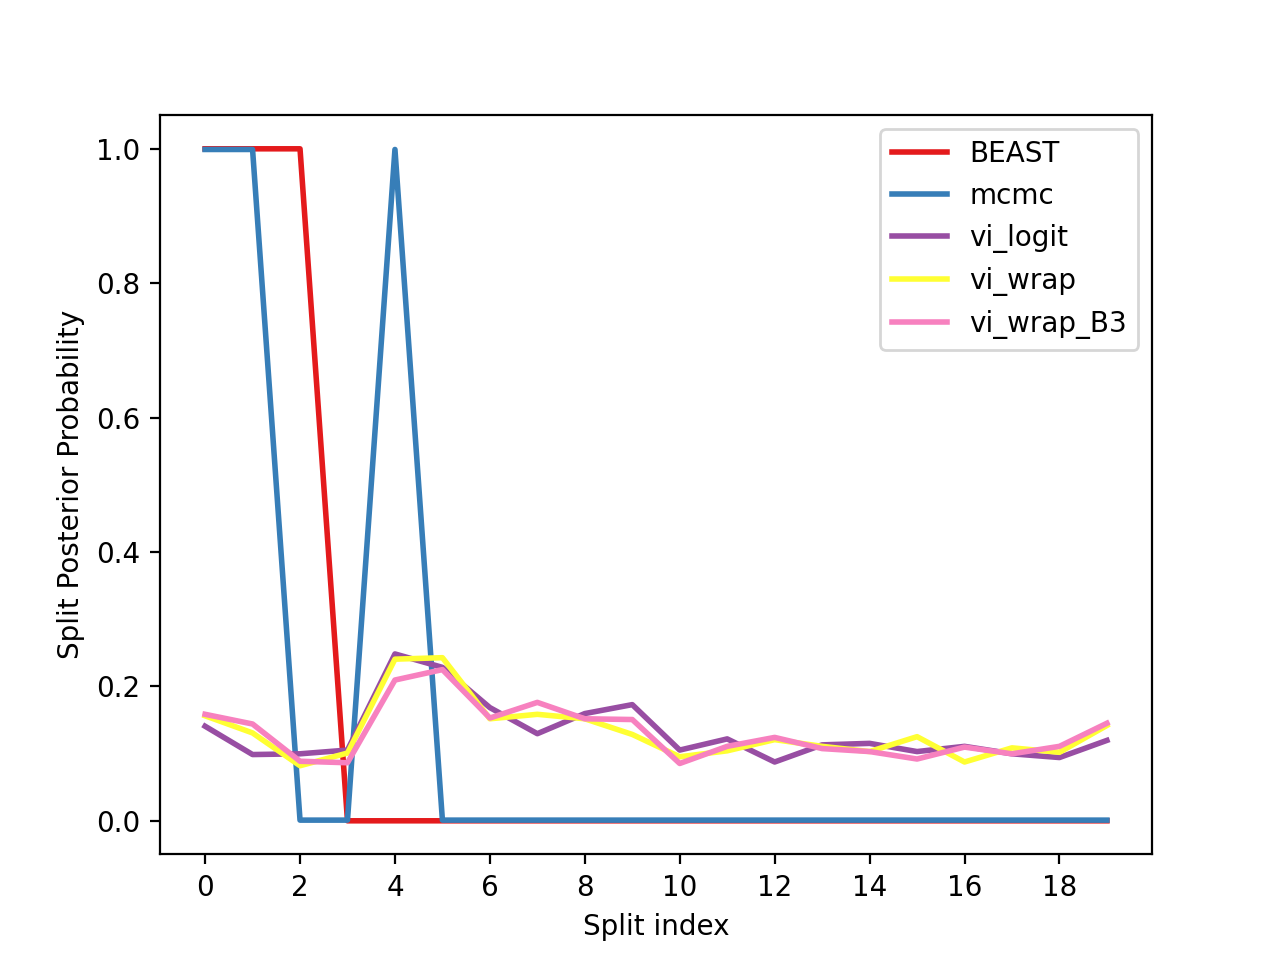
\includegraphics[width=.333\linewidth]{fig/cmp_splits}%
\includegraphics[width=.333\linewidth]{fig/cmp_tree_length}%
\includegraphics[width=.333\linewidth]{fig/cmp_treeness}
\includegraphics[width=.25\linewidth]{fig/cmp_b1}%
\includegraphics[width=.25\linewidth]{fig/cmp_b2}%
\includegraphics[width=.25\linewidth]{fig/cmp_b3}%
\includegraphics[width=.25\linewidth]{fig/cmp_b4}
\caption{Comparison of tree statistics between Beast and Dodonaphy: (a) split posterior probability (b) total branch length (c) ``treeness'' (signal/signal+noise) (d-g) branch lengths (possibly not same branch??).}
\label{fig:stat_cmp}
\end{center}
\end{figure}

Figure~\ref{fig:locations} shows a kernel density estimate for each node location at various stages.
Comparing figures~\ref{fig:locations}a and b reveals that the posterior surface of nodes can drift over the simulation.
Indeed tree reconstructions are invariant to isometries on the embedded points since they are only based on their relative distances.
Additionally, tree reconstructions won't change as a tip node moves along the surface with constant distance to its nearest neighbour (provided the tree doesn't change topology).
The embedded posterior surfaces generated from samples $\bold{X}_{i}$ shouldn't be considered static, but transient over the simulation.
Nonetheless, these degrees of freedom should not affect the result of the MCMC.

These densities are clearly not normally distributed.
The feasibility of VI rests on how well a simple distribution $q$ can approximate these densities.
Boosting to a mixture model may increase the ability for VI to represent these embeddings.
	
\subsection{VI}
The traces in figure~\ref{fig:elbos} illustrate that the elbos has a strange start, getting worse for a few hundred epochs, but then increases steadily but probably hasn’t converged after the 1e4 epochs.
\begin{figure}[htbp]
\begin{center}
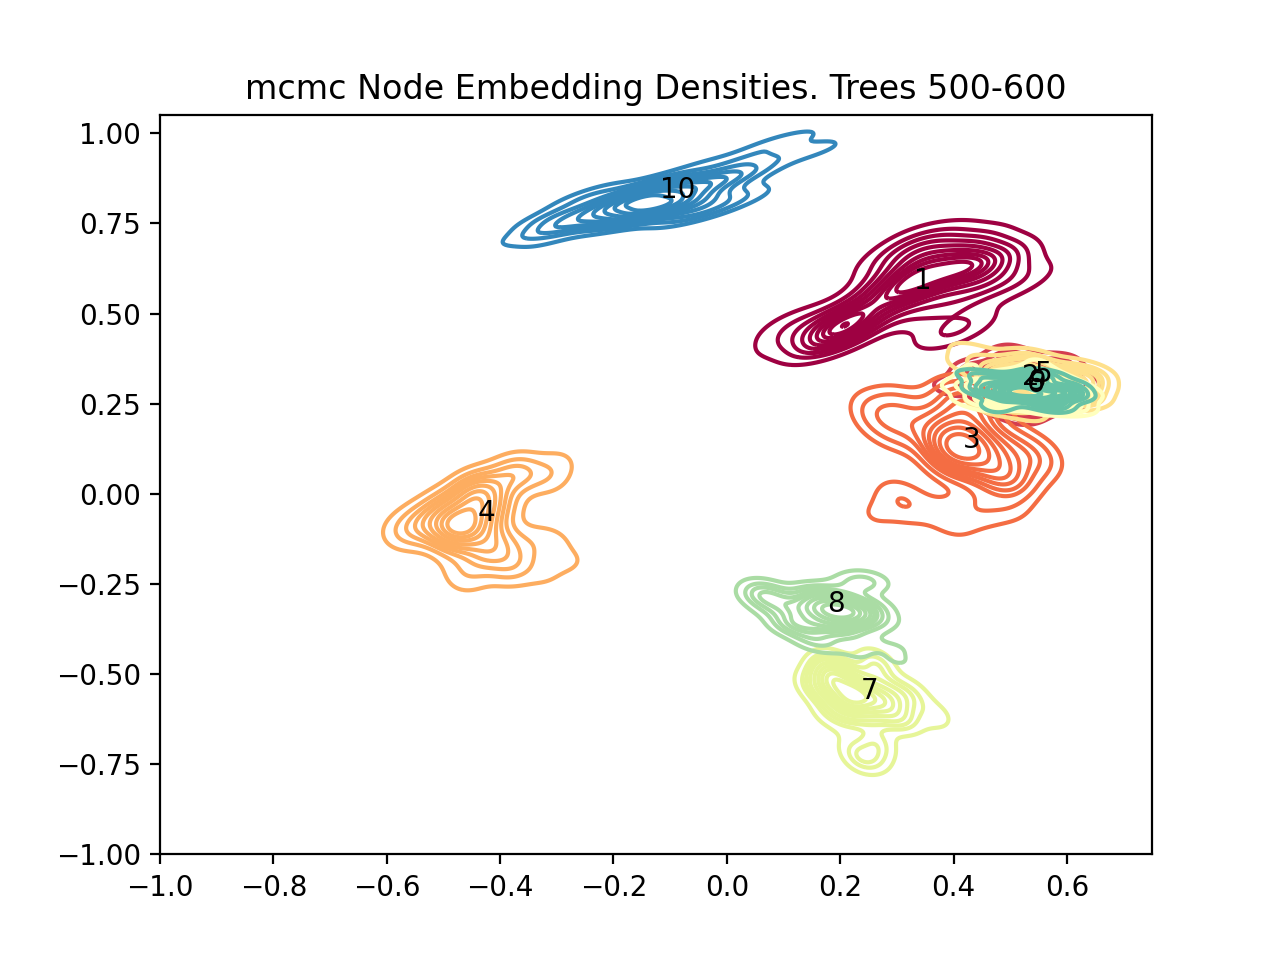
\includegraphics[width=.5\linewidth]{fig/locations_500.png}%
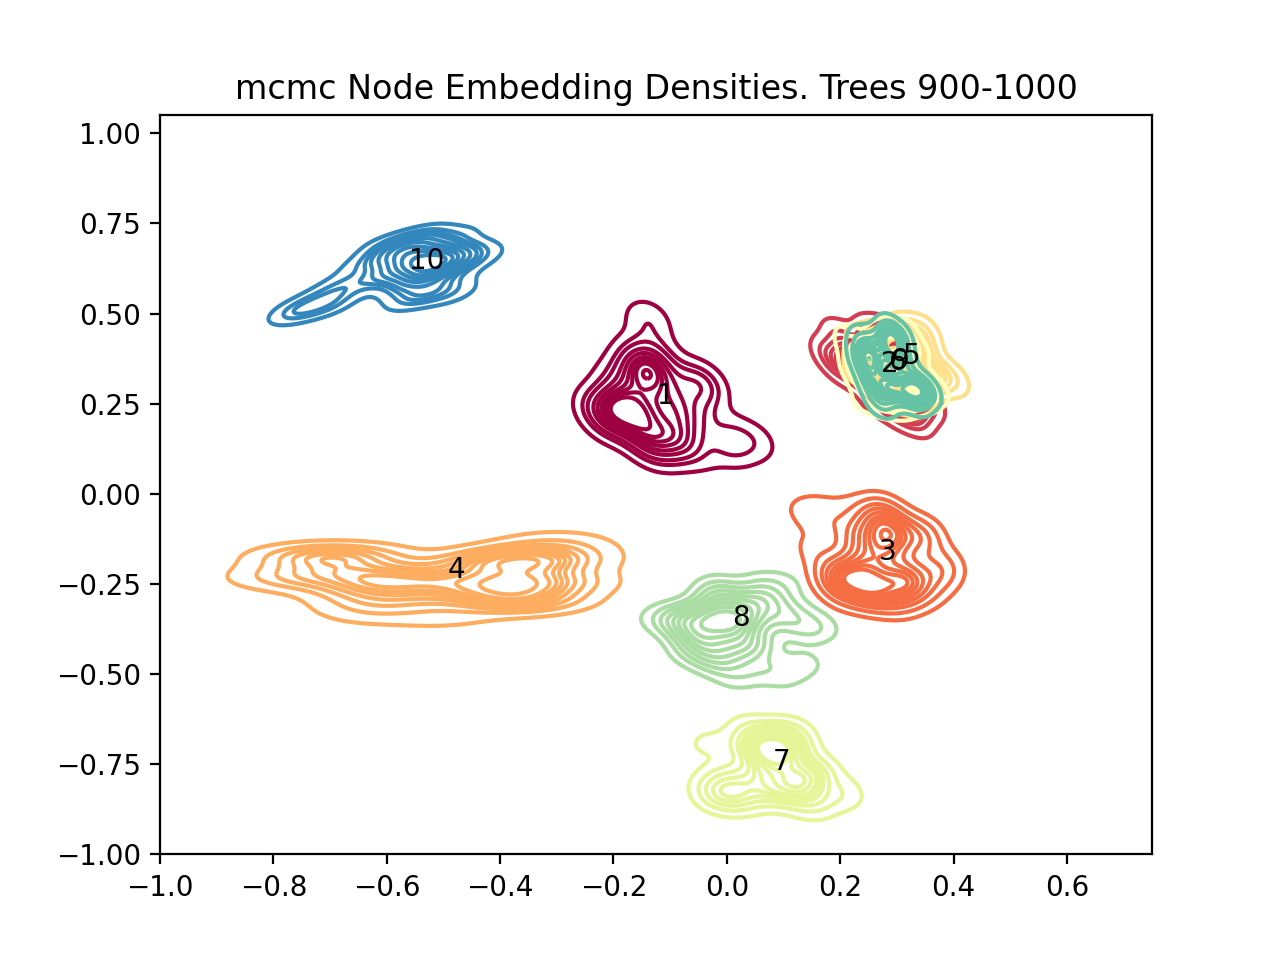
\includegraphics[width=.5\linewidth]{fig/locations_900.png}
\includegraphics[width=.5\linewidth]{fig/VI_params_init.png}%
\includegraphics[width=.5\linewidth]{fig/VI_params.png}
\includegraphics[width=.5\linewidth]{fig/geo_params_init.png}%
\includegraphics[width=.5\linewidth]{fig/geo_params.png}
\caption{Density estimates of the node locations from Dodonaphy's MCMC projected into $\mathbb{R}^{2}$. (a) Tree 500-600 and (b) 900-1000 in the sampled MCMC chain. On a different data set: (c) initial variational densities in $\mathbb{P}^{2}$ using a truncated exponential on internal node radius. The binary MST depicted, uses the mean of each node's density. (d) After learning for $10^{4}$ epochs. (e-f) Same as above but using the geodesics method.}
\label{fig:elbos}
\end{center}
\end{figure}

\begin{figure}[htbp]
\begin{center}
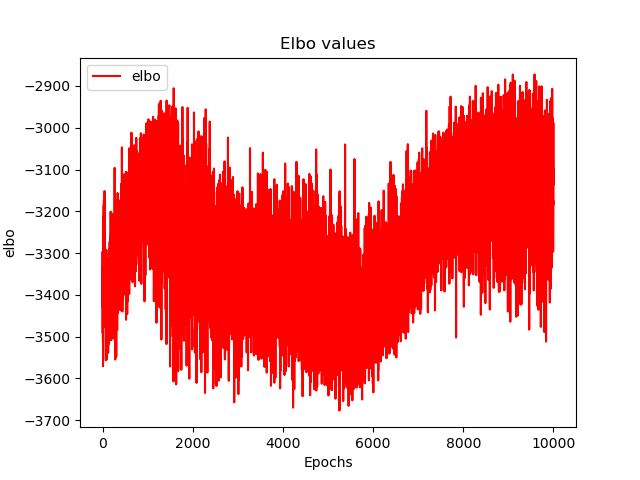
\includegraphics[width=.333\linewidth]{fig/elbo_trace_logit.png}%
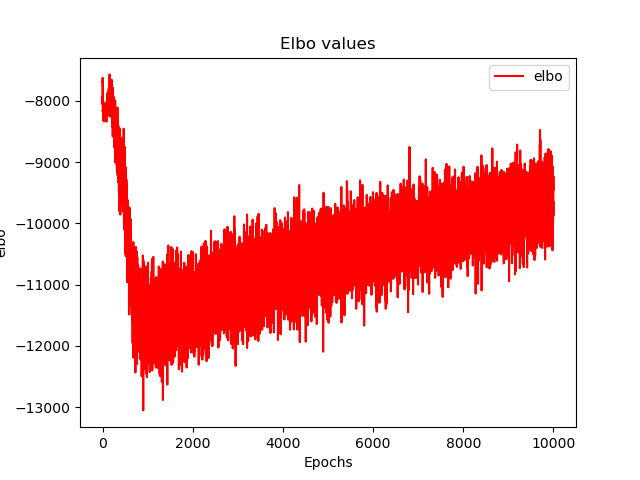
\includegraphics[width=.333\linewidth]{fig/elbo_trace_wrap.png}%
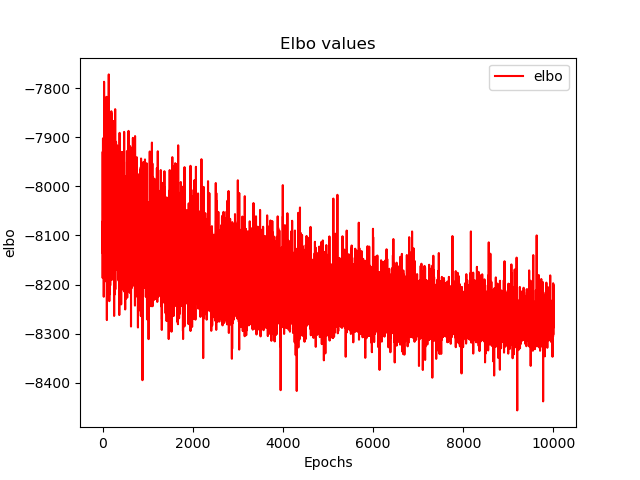
\includegraphics[width=.333\linewidth]{fig/elbo_trace_wrap_B3.png}
\includegraphics[width=.333\linewidth]{fig/elbo_trace_k10.png}%
\includegraphics[width=.333\linewidth]{fig/elbo_trace_wrap2.png}%
\includegraphics[width=.333\linewidth]{fig/elbo_trace_geo.png}
\caption{ELBO trace from VI on six taxa using (a) the logit method, (b) the wrapping method and (c) the wrapping method using a mixture of three Gaussians. Simulation used $10^{4}$ epochs, $n=2$ dimensions and $k=10$ samples to evaluate the elbo. Final ELBOs were (a) $-9539$, (b) $-9690$ and (c) -8264. Second row shows analysis of second data set using (d) logistic method, (e) wrapping method (f) logistic method with geodesics.}
\label{fig:elbo}
\end{center}
\end{figure}

\begin{figure}[htbp]
\begin{center}
\includegraphics[width=.333\linewidth]{fig/elbo_trace_k1.png}%
\includegraphics[width=.333\linewidth]{fig/elbo_trace_k10.png}%
\includegraphics[width=.333\linewidth]{fig/elbo_trace_k100.png}
\caption{Effect of number of ELBO samples $k=\{1, 10, 100\}$.}
\label{fig:k_samples}
\end{center}
\end{figure}

\begin{figure}[htbp]
\begin{center}
\includegraphics[width=.333\linewidth]{fig/elbo_trace_lr1.png}%
\includegraphics[width=.333\linewidth]{fig/elbo_trace_lr01.png}%
\includegraphics[width=.333\linewidth]{fig/elbo_trace_lr0001.png}
\caption{Effect of learning rate $\{1, 10^{-1}, 10^{-4}\}$.}
\label{fig:lr}
\end{center}
\end{figure}

\begin{figure}[htbp]
\begin{center}
\includegraphics[width=.333\linewidth]{fig/elbo_trace_SGD.png}%
\includegraphics[width=.333\linewidth]{fig/elbo_trace_d3.png}%
\includegraphics[width=.333\linewidth]{fig/elbo_trace_b3.png}
\caption{Trying (a) SGD instead of Adam. (b) 3-dimensions. (c) Boosting with a mixture of 3 Gaussians.}
\label{fig:lr}
\end{center}
\end{figure}


\section{Thoughts}
\subsection{MCMC}
\begin{itemize}
\item Try other (Chami) method of connecting?
\item What type of tree rearrangements commonly occur?
\item Is likelihood under JC69 continuous when topology changes?
\item If the nodes move without changing the topology, is the posterior probability smooth?
\item Hot chain/ MCMCMC?
\end{itemize}

\subsection{VI}
\begin{itemize}
\item What if we learn the curvature?
\item Effect of $k_{samples}$, boosts, learning rate?
\item How easy is it to add taxa? Might only need pair-wise distance to a subset of other taxa.
\item We could use the original parameterisation with the radius in $r \sim P(N(\mu, \sigma))$ a logit-normal distribution and the directional similarly in a $n$-dimensional logit-normal.
\end{itemize}

\subsection{Full rank}
Intuitively, nodes that are close together should be a bit correlated. However, it doesn't seem to improve things much. In the off-diagonals in the covariance matrix are initialised to zero, the ELBO gets much higher faster compared to if the off-diagonal terms have a non-zero covariance. That said, I haven't run simulations long enough to be sure, only $1000$ epochs with a small learning rate of $0.01$.

\subsection{Distance-based}
Could we adopt an approach like Wilson and Chami, where only the distributions of the embedded points are optimised based on their pair-wise distances.
Only then do we infer a tree.
The advantage of this is that the cost function is differentiable and more in line with what other people in the ML community do.
However, this isn't actually modelling the Bayesian Posterior, just a proxy for it.

Tips are labelled, internal nodes are not.

\section{Appendix}
\subsection{Numerical stability in Hyperbolic space}
As either $||x||_{2}^{2}\to 1$ or $||y||_{2}^{2} \to 1$, eq.~\ref{eq:poin_dist} can become a numerically unstable way to compute distances.
Since the poincare ball is a stereographic projection of the hyperboloid, an equivalent metric comes from projecting of $x$ and $y$ into the hyperboloid model of $\mathbb{H}^{d}$ and using its metric.
The hyperboloid model is the sheet inside $\bold{x}\in\mathbb{R}^{d+1}$ such that $x_{0}^{2} - \sum_{i} x_{i}^{2} = 1$.
It has metric $d_{hyp}(\bold{x}, \bold{y}) = \text{acosh}(-\langle \bold{x}, \bold{y} \rangle)$, where the Lorentz inner product of $\bold{x}$ and $\bold{y}$ is:
\begin{equation*}
	\langle \bold{x}, \bold{y} \rangle = -x_{0}y_{0} + \sum_{i>0} x_{i}y_{i}
\end{equation*}
The stereographic projection onto the hyperboloid $\phi:\mathbb{P}^{d} \to \mathbb{H}^{d}$ takes a point to $\psi(\bold{x}) = \big(\frac{(1+||x||_{2})}{(1-||x||_{2})}, \frac{2 \bold{x}}{(1- ||x||_{2}}\big)$.
Thus, for $\bold{x}, \bold{y} \in \mathbb{P}_{d}$ we can use $d(\bold{x}, \bold{y}) = d_{hyp}(\psi(\bold{x}), \psi(\bold{y}))$.

% define \Phi inverse explicitly in







\end{document}